\doublespacing{}
\setlength{\parindent}{4ex}
\chapter{Introduction}
Once the whole thesis is done, here I want to explain the structure of the thesis.

\section{What is cryptography}
\par The definition of cryptography given in the Webster dictionary is ``\textit{secret writing}''. This is historically precise, since in ancient times, people apply the idea of cryptography solely to enable secret communication. Most ancient cryptography schemes, as well as some modern ones look like some kind of puzzle. Yet creating and breaking the scheme would rely on how well you can manipulate the puzzle. Substitution cipher, which replaces each unit of the plaintext to a ciphertext, can be considered as a significant example of puzzle-like encryption. Assume that we are working with English, in this case, unit of plaintext will be each letter.
\begin{figure}[h]
    \centering
    \setlength\tabcolsep{3pt}
        \begin{tabular}{cccccccccccccccccccccccccc}
        A & B & C & D & E & F & G & H & I & J & K & L & M & N & O & P & Q & R & S & T & U & V & W & X & Y & Z \\
        $\downarrow$ & $\downarrow$ & $\downarrow$ & $\downarrow$ & $\downarrow$ & $\downarrow$ & $\downarrow$ & $\downarrow$ & $\downarrow$ & $\downarrow$ & $\downarrow$ & $\downarrow$ & $\downarrow$ & $\downarrow$ & $\downarrow$ & $\downarrow$ & $\downarrow$ & $\downarrow$ & $\downarrow$ & $\downarrow$ & $\downarrow$ & $\downarrow$ & $\downarrow$ & $\downarrow$ & $\downarrow$ & $\downarrow$ \\
        Z & E & B & R & A & S & C & D & F & G & H & I & J & K & L & M & N & O & P & Q & T & U & V & W & X & Y \\
    \end{tabular}
    \caption{Map letter to letter.}
    \label{fig:replace-letter-by-letter}
\end{figure}
One trivial example could be substitute each letter to another unique letter like shown in Figure~\ref{fig:replace-letter-by-letter}. If we encrypt the sentence \textit{``life is like a box of chocolates''} with the relations specified in Figure~\ref{fig:replace-letter-by-letter}, we get \textit{``ifsafpifhazelwlsbdlblizqap''} back as the ciphertext. Correspondences between plaintext and ciphertext can be very creative as long as the communicating parties hold the same information. The ``creative'' example is shown in Figure~\ref{fig:replace-letter-by-icon}, where we are replacing letters by icons which are completely irrelevant.
\begin{figure}[h]
    \centering
    \setlength\tabcolsep{3pt}
    \begin{tabular}{cccccccc}
        A & B & C & D & E & $\cdots$ & Y & Z \\
        $\downarrow$ & $\downarrow$ & $\downarrow$ & $\downarrow$ & $\downarrow$ & $\cdots$ &$\downarrow$ &$\downarrow$ \\
        \faBinoculars{} & \faCube{} & \faEnvelope{} & \faFighterJet{} & \faGift{} & $\cdots$ & \faHeart{} & \faInstitution{} \\
    \end{tabular}
    \caption{Map letter to icon.}
    \label{fig:replace-letter-by-icon}
\end{figure}
Intuitively, we know the security of substitution cipher is based on the fact that the correspondence between plaintext and ciphertext is unknown to the attacker. In general, we would say the more abstract the substitution is, the less likely for someone who doesn't know the correspondence to break the substitution cipher.
\par What else worth mentioning is that, in history, the biggest motivation for people to research in this field and in fact, most applications of this field were military related. Thus the term cryptography seemed far away from people's daily life. However, cryptography has largely changed since the invention of computers and the internet. It has merged deeply into our daily life though you may not have noticed. Every time when you log in your email account or when you purchase an item from an online shop, you have undoubtedly used cryptography. While you communicating with the web servers, your email account password or credit card number will first be encrypted and then send through the networks. If those important information was never encrypted, anyone who have the ability to monitor your network will be able to retrieve them.
\par While we cannot deny securing communication is still a major functionality of cryptography, the study of cryptography has developed other branches that are equally as important. Some of the noticeable branches that modern cryptography involves are key exchanging protocols, message authentication methods, hash functions and more.
\par One of the other thing computers brought to us is the ample computational powers. In modern times, a 30 dollars Raspberry Pi can do an exhaustive attack on the substitution cipher on 26 English letters in the time it takes to make a cup of coffee. Thus, deviating from studying the art of clever puzzles, modern cryptography makes extensive use of mathematics, including fields such as abstract algebra, number theory, statistics, combinatorics and computational complexities. Modern cryptography protocols are designed around some computational hardness assumptions.
\par In a nutshell, cryptography has gone from the set of clever puzzles concerned with ensuring secret communication for the military to a science that provides security for ordinary people across the globe.

\section{Rubik's cube and cryptography}
% ---------------------- Figure for a solved rubik's cube ----------------------
\begin{wrapfigure}{r}{6cm}
    \centering
    \RubikCubeSolved{}
    \ShowCube{5cm}{0.7}{\DrawRubikCubeLU}
    \caption{A solved rubik's cube.}
    \label{fig:solved-cube}
\end{wrapfigure}
% ------------------------------------------------------------------------------
\par Rubik's cube, as shown in Figure~\ref{fig:solved-cube}, is a three dimensional puzzle invented in 1974 by Hungarian professor Ernő Rubik. The most common Rubik's cube has six faces. The faces of the cube are covered by the following solid colors: white, red, blue, yellow, orange and green. For a solved cube, the white face is always opposite to the yellow face, red is opposite to orange and blue is opposite to green. In Figure~\ref{fig:solved-cube}, the Rubik's cube has three small cubes on each side. We say that this is a 3 by 3 by 3 cube. Clearly each face of the cube includes nine squares. In future discuss, we will call those squares ``cubies''.
\par After years of developing, Rubik's cubes now exist in many forms. For the six faced cubes, their side lengths may vary from 2 to 13 or even larger number. However, since their structures are similar, they share a lot of properties in common. That is to say that no matter the side length, all six faced cubes can be solved in an almost identical fashion.
\begin{figure}[h]
    \centering
    \begin{minipage}{0.45\textwidth}
        \centering
        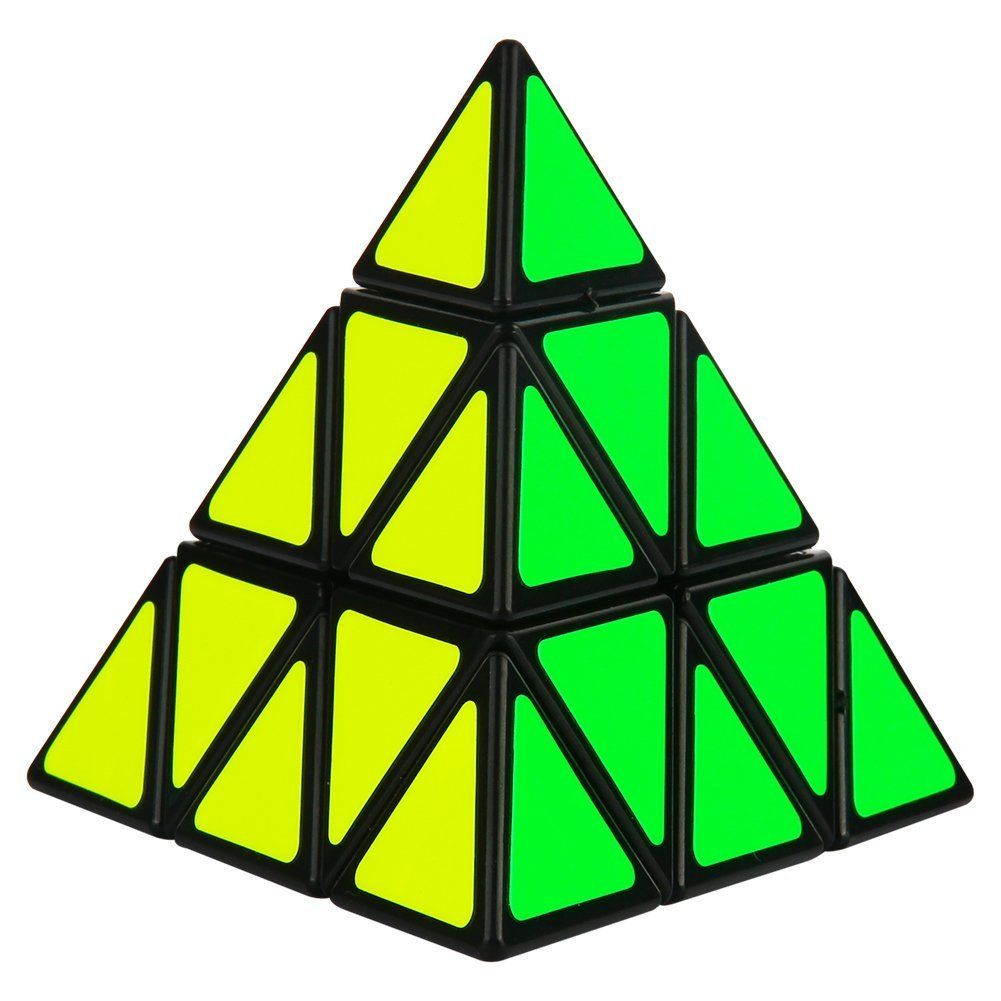
\includegraphics[width=.6\linewidth]{figures/pyraminx_cube.jpg}
        \caption{A solved pyraminx cube.}
        \label{fig:pyraminx-cube}
    \end{minipage}
    \begin{minipage}{0.45\textwidth}
        \centering
        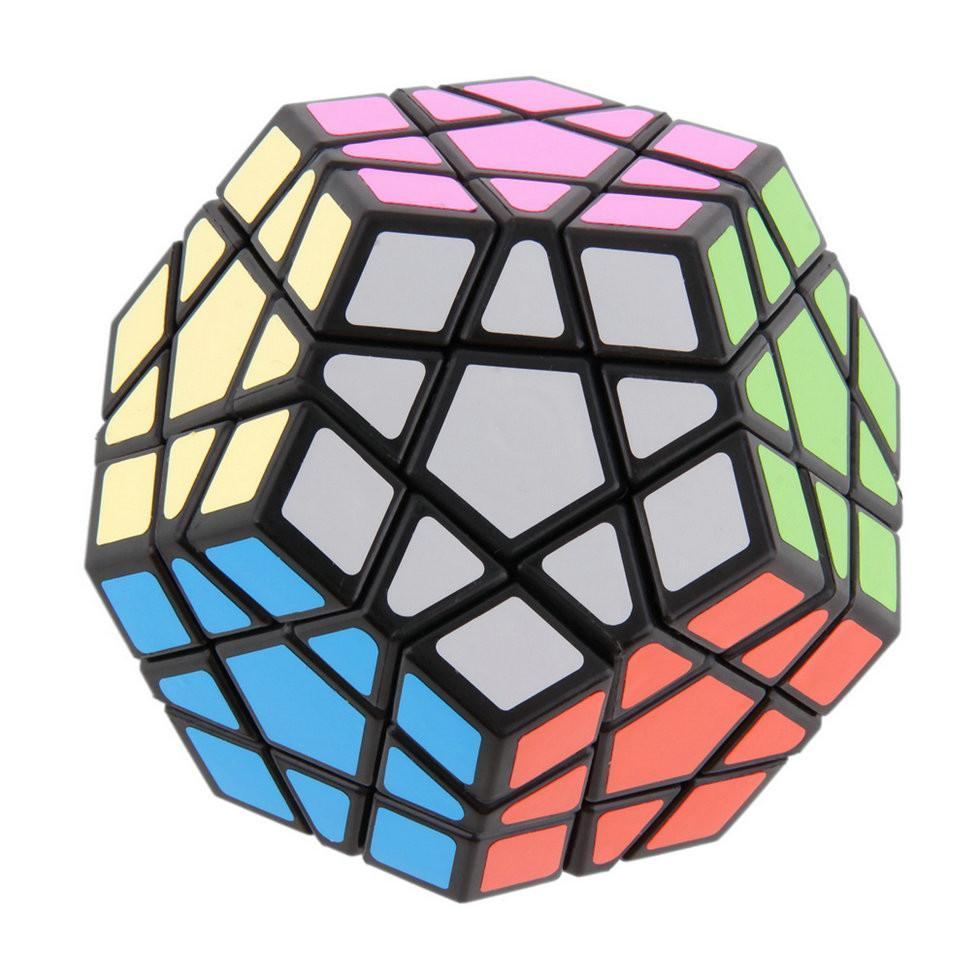
\includegraphics[width=.6\linewidth]{figures/pentagon_cube.jpg}
        \caption{A solved pentagon cube.}
        \label{fig:pentagon-cube}
    \end{minipage}
\end{figure}
Rubik's cubes also have other structures; ``cubes'' with four or twelve faces have also been made in production.
\par Why would we relate Rubik's cubes and cryptography? \todo[size=\tiny]{Will need to clarify somewhat when we have more of the thesis outlined} Obviously, Rubik's cubes provide a good shuffling scheme, and Rubik's cubes are known to be hard to solve. One may argue that this is not true, since the best human players can solve a 3 by 3 by 3 cube in about 6 seconds. By following the developed algorithms, anyone can solve a well shuffled Rubik's cube within minutes. Let's consider each different shuffling result of the Rubik's cube as a state. It is true that Rubik's cubes have a lot of different states. The most common 3 by 3 by 3 Rubik's cube has over 43 quintillion different states. It will take hundreds of years for a powerful desktop to run through all of them. Being such a powerful device, we know that a scheme designed based on Rubik's cubes could be safe against exhaustive search attacks. In addition, we can view Rubik's cubes as groups. The nice properties of groups are widely used in cryptography. We will explore more about this in the following chapters.

\section{Preliminaries}
\par First let's take a look at \textbf{\textit{Kerckhoffs’ principle}}:
\begin{quote}
    \textit{The cipher method must not be required to be secret, and it must be able to fall into the hands of the enemy without inconvenience.}
\end{quote}
This principle tells us that the security of one encryption protocol does not rely on the encryption protocol procedures being unknown. One may wonder how do we obtain the security while the eavesdropper knows all the details. But there is one thing the eavesdropper does not know, which is the \textbf{\textit{key}}. In fact, security of all classical encryption schemes depend on the key shared by the communicating parties being unknown by the eavesdropper. For the previous example, substitution cipher, we can consider the correspondence between plaintext and ciphertext as the key. As we said, the security of substitution cipher depends on the key being secret. This scenario is known as the private-key setting. Under this setting, we will introduce some cryptography syntax.
\par Formally, to create a private-key encryption scheme, we need to specify a message space $\mathcal{M}$. This message space $\mathcal{M}$ defines the set of ``legal'' messages. Taking the substitution cipher described in Figure~\ref{fig:replace-letter-by-letter} as an example, a ``legal'' message could be any combination of English letters, regardless of if it has any actual meaning. In contrast, containing a Greek letter will make the message  ``illegal''. Along with defining the key space, we need three algorithms for the encryption scheme. They are \textbf{Gen}, \textbf{Enc} and \textbf{Dec}. The functionalities of the algorithms are the following:
\begin{itemize}
    \item \textbf{Gen} is the procedure for generating keys. It is a probabilistic algorithm that outputs a key $k$ with desired length according to some distribution (usually, the normal distribution).
    \item \textbf{Enc} is the procedure for encrypting the message. In the private-key encryption scheme, it takes a key $k$ and a message $m \in \mathcal{M}$ as inputs. Then it use $k$ to encrypt $m$ and outputs ciphertext $c$. We denote this process by \textbf{Enc}$_k(m)$.
    \item \textbf{Dec} is the procedure for decrypting the message. In the private-key encryption scheme, it takes a key $k$ and a ciphertext $c$ as inputs. Then it use $k$ to decrypt $c$ and outputs plaintext $m$. We denote this process by \textbf{Dec}$_k(c)$.
\end{itemize}
\begin{definition} \textbf{The correctness of an encryption scheme.} \\
    For any encryption scheme $\Pi$, for every $k$ generated by \textbf{Gen} and every message $m \in \mathcal{M}$, it must hold that \[\textbf{Dec}_k(\textbf{Enc}_k(m)) = m\]
\end{definition}
